\documentclass{article}
\usepackage[hyphens]{url}
\usepackage{mathtools}
\usepackage{amsmath}
\usepackage{listings}
\usepackage{graphicx}
\usepackage[margin=1in]{geometry}
\usepackage{float}
\floatstyle{boxed}
\restylefloat{figure}
\lstset{basicstyle=\footnotesize, breaklines=true}
\begin{document}


\title{CS595 Intro to Web Science, Assignment \#9}
\author{Valentina Neblitt-Jones}
\date{December 5, 2013}
\maketitle

\newpage
\listoftables
\lstlistoflistings
\listoffigures

\newpage
\section*{Question 1}

Create a blog-term matrix. Start by grabbing 100 blogs; include: \\

\begin{itemize}
\item \url{http://f-measure.blogspot.com/}
\item \url{http://ws-dl.blogspot.com/}
\end{itemize}

and grab 98 more as per the method shown in class. \\

Use the blog title as the identifier for each blog (and row of the matrix). Use the terms from every item/title (RSS) or entry/title (Atom) for the columns of the matrix. The values are the frequency of occurrence. Essentially you are replicating the format of the ``blogdata.txt'' file included with the PCI book code. Limit the number of terms to the most ``popular'' (i.e., frequent) 500 terms, this is \textbf{after} the criteria on p. 32 (slide 7) has been satisfied.

\subsection*{Answer to Question 1}
Use the book here \cite{pci}

\newpage
\section*{Question 2}
Create an ASCII and JPEG dendrogram that clusters (i.e., HAC) the most similar blogs (see slides 12 \& 13). Include the JPEG in your report and upload the ASCII file to GitHub (it will be too unwieldy for inclusion in the report.)

\subsection*{Answer to Question 2}


\newpage
\section*{Question 3}
Cluster the blogs using K-Means, using k=5, 10, 20 (see slide 18). How many iterations were required for each value of k?

\subsection*{Answer to Question 3}


\newpage
\section*{Question 4}
Use MDS to create a JPG of the blogs similar to slide 29. How many iterations were required?

\subsection*{Answer to Question 4}

\newpage
\section*{Question 5 - Extra Credit (5 points)}
Re-run Q2, but this time with proper TFIDF calculations instead of the hack discussed on slide 7 (p. 32). Use the same 500 words, but this time replace their frequency count with TFIDF scores as computed in assignment \#3. Document the code, techniques, methods, etc. used to generate these TFIDF values. Upload the new file to GitHub. \\

Compare and contrast the resulting dendrogram with the dendrogram from Q2. \\

Note: Ideally you would not reuse the same 500 terms and instead come up with TFIDF scores for all the terms and choose the top 500 from that list, but I am trying to limit the amount of work necessary.

\subsection*{Answer to Question 5}

Use the book here \cite{pci}

%\renewcommand\thesubsection{\arabic{subsection}}
%\subsection{What 5 movies have the highest average ratings? Show the movies and their ratings sorted by their average ratings.}

%\begin{lstlisting}[frame=single, caption=highestavgrating.py, label=highaverage]
%\end{lstlisting}

%\newpage
%\subsection{What 5 movies have received the most ratings? Show the movies and the number of ratings sorted by number of ratings.}

%\begin{table}[!h]
%\centering
%\begin{tabular}{l c}
%Movie Title & No. of Ratings \\
%\hline
%Star Wars (1977) & 583  \\
%Contact (1997) & 509  \\
%Fargo (1996) & 508  \\
%Return of the Jedi (1983) & 507  \\
%Marlene Dietrich: Shadow and Light (1997) & 485  \\
%\hline
%\end{tabular}
%\caption{Movies with the Most Ratings}
%\end{table}

%\begin{figure}[H]
%\centering
%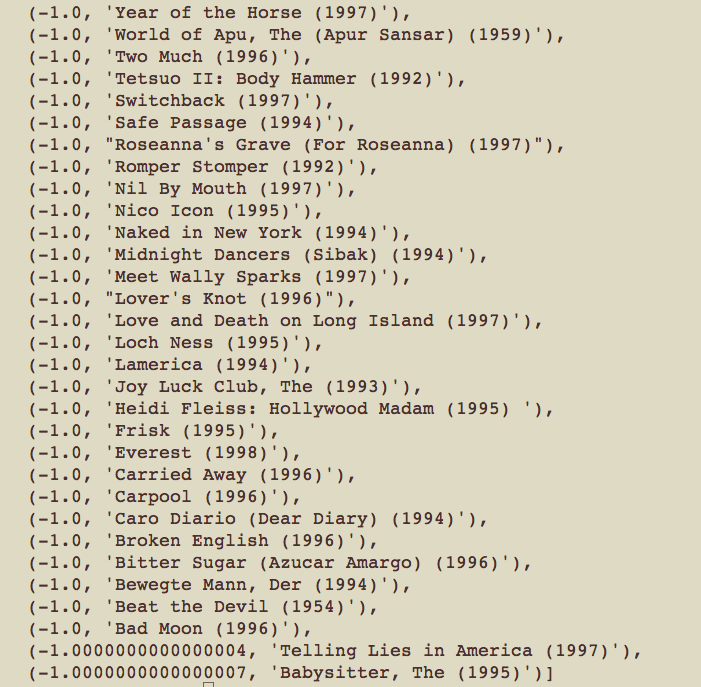
\includegraphics[scale=0.50]{q05/leastliketopgun}
%\caption{Movies Least Like Top Gun}
%\label{leastliketopgun}
%\end{figure}

\newpage
\appendix
\section{Appendix Title}

%\begin{lstlisting}[frame=single, caption=recommendations.py, label=recommendations]
%\end{lstlisting}

\newpage

\bibliographystyle{acm}
\bibliography{references}

\end{document}